\documentclass[12pt,a4paper,parskip]{scrartcl}
\usepackage[utf8]{inputenc}
\usepackage[T1]{fontenc}
\usepackage[ngerman]{babel}
\usepackage{lmodern}
\usepackage[babel,german=guillemets]{csquotes}
\usepackage[style=verbose-ibid,backend=bibtex8]{biblatex}
\bibliography{baclit110414}
\usepackage{amsmath}
\usepackage{amsfonts}
\usepackage{amssymb}
\usepackage{makeidx}
\usepackage{graphicx}
\usepackage{url}
\usepackage[locale=DE]{siunitx}%SI Einheiten etc.
\usepackage[german]{fancyref}%möglicherweise rausnehmen oder justieren
\usepackage{booktabs} %Tabellen Horizontale Linier dick darstellen
\usepackage{rotating}
\usepackage{lscape}
\usepackage{subfig}
\usepackage{here}
\usepackage{color}
\usepackage[left=3cm,right=3cm,top=2cm,bottom=2cm]{geometry}
\usepackage{mdwlist}
\begin{document}
\author{Benedikt Kaffanke}
\title{Protokoll und Annahmen zum manuellen Schleifen und Polieren}
\maketitle
\newpage
\tableofcontents
\subsection{Vorgehensweise}
Aufgrund von Engpässen in der Serienfertigung war es nicht möglich die Materialchargen F17, Fxx und F18 auf modernen Taktanlagen schleifen und polieren zu lassen. Deshalb wurde für diese Bearbeitungsstufe ein Handwerksbetrieb beauftragt. Um Erkenntnisse über die Oberflächentemperaturen des Bauteils während der Bearbeitung zu bekommen, wurden die Teile von innen mit Temperaturmessstreifen versehen (siehe \fref{fig:messaction}). Weiterhin wurde, um Schmelzkreide aufzutragen, während des Polierens das Werkstück kurz weggeschwenkt.

\begin{figure}[H]
\centering
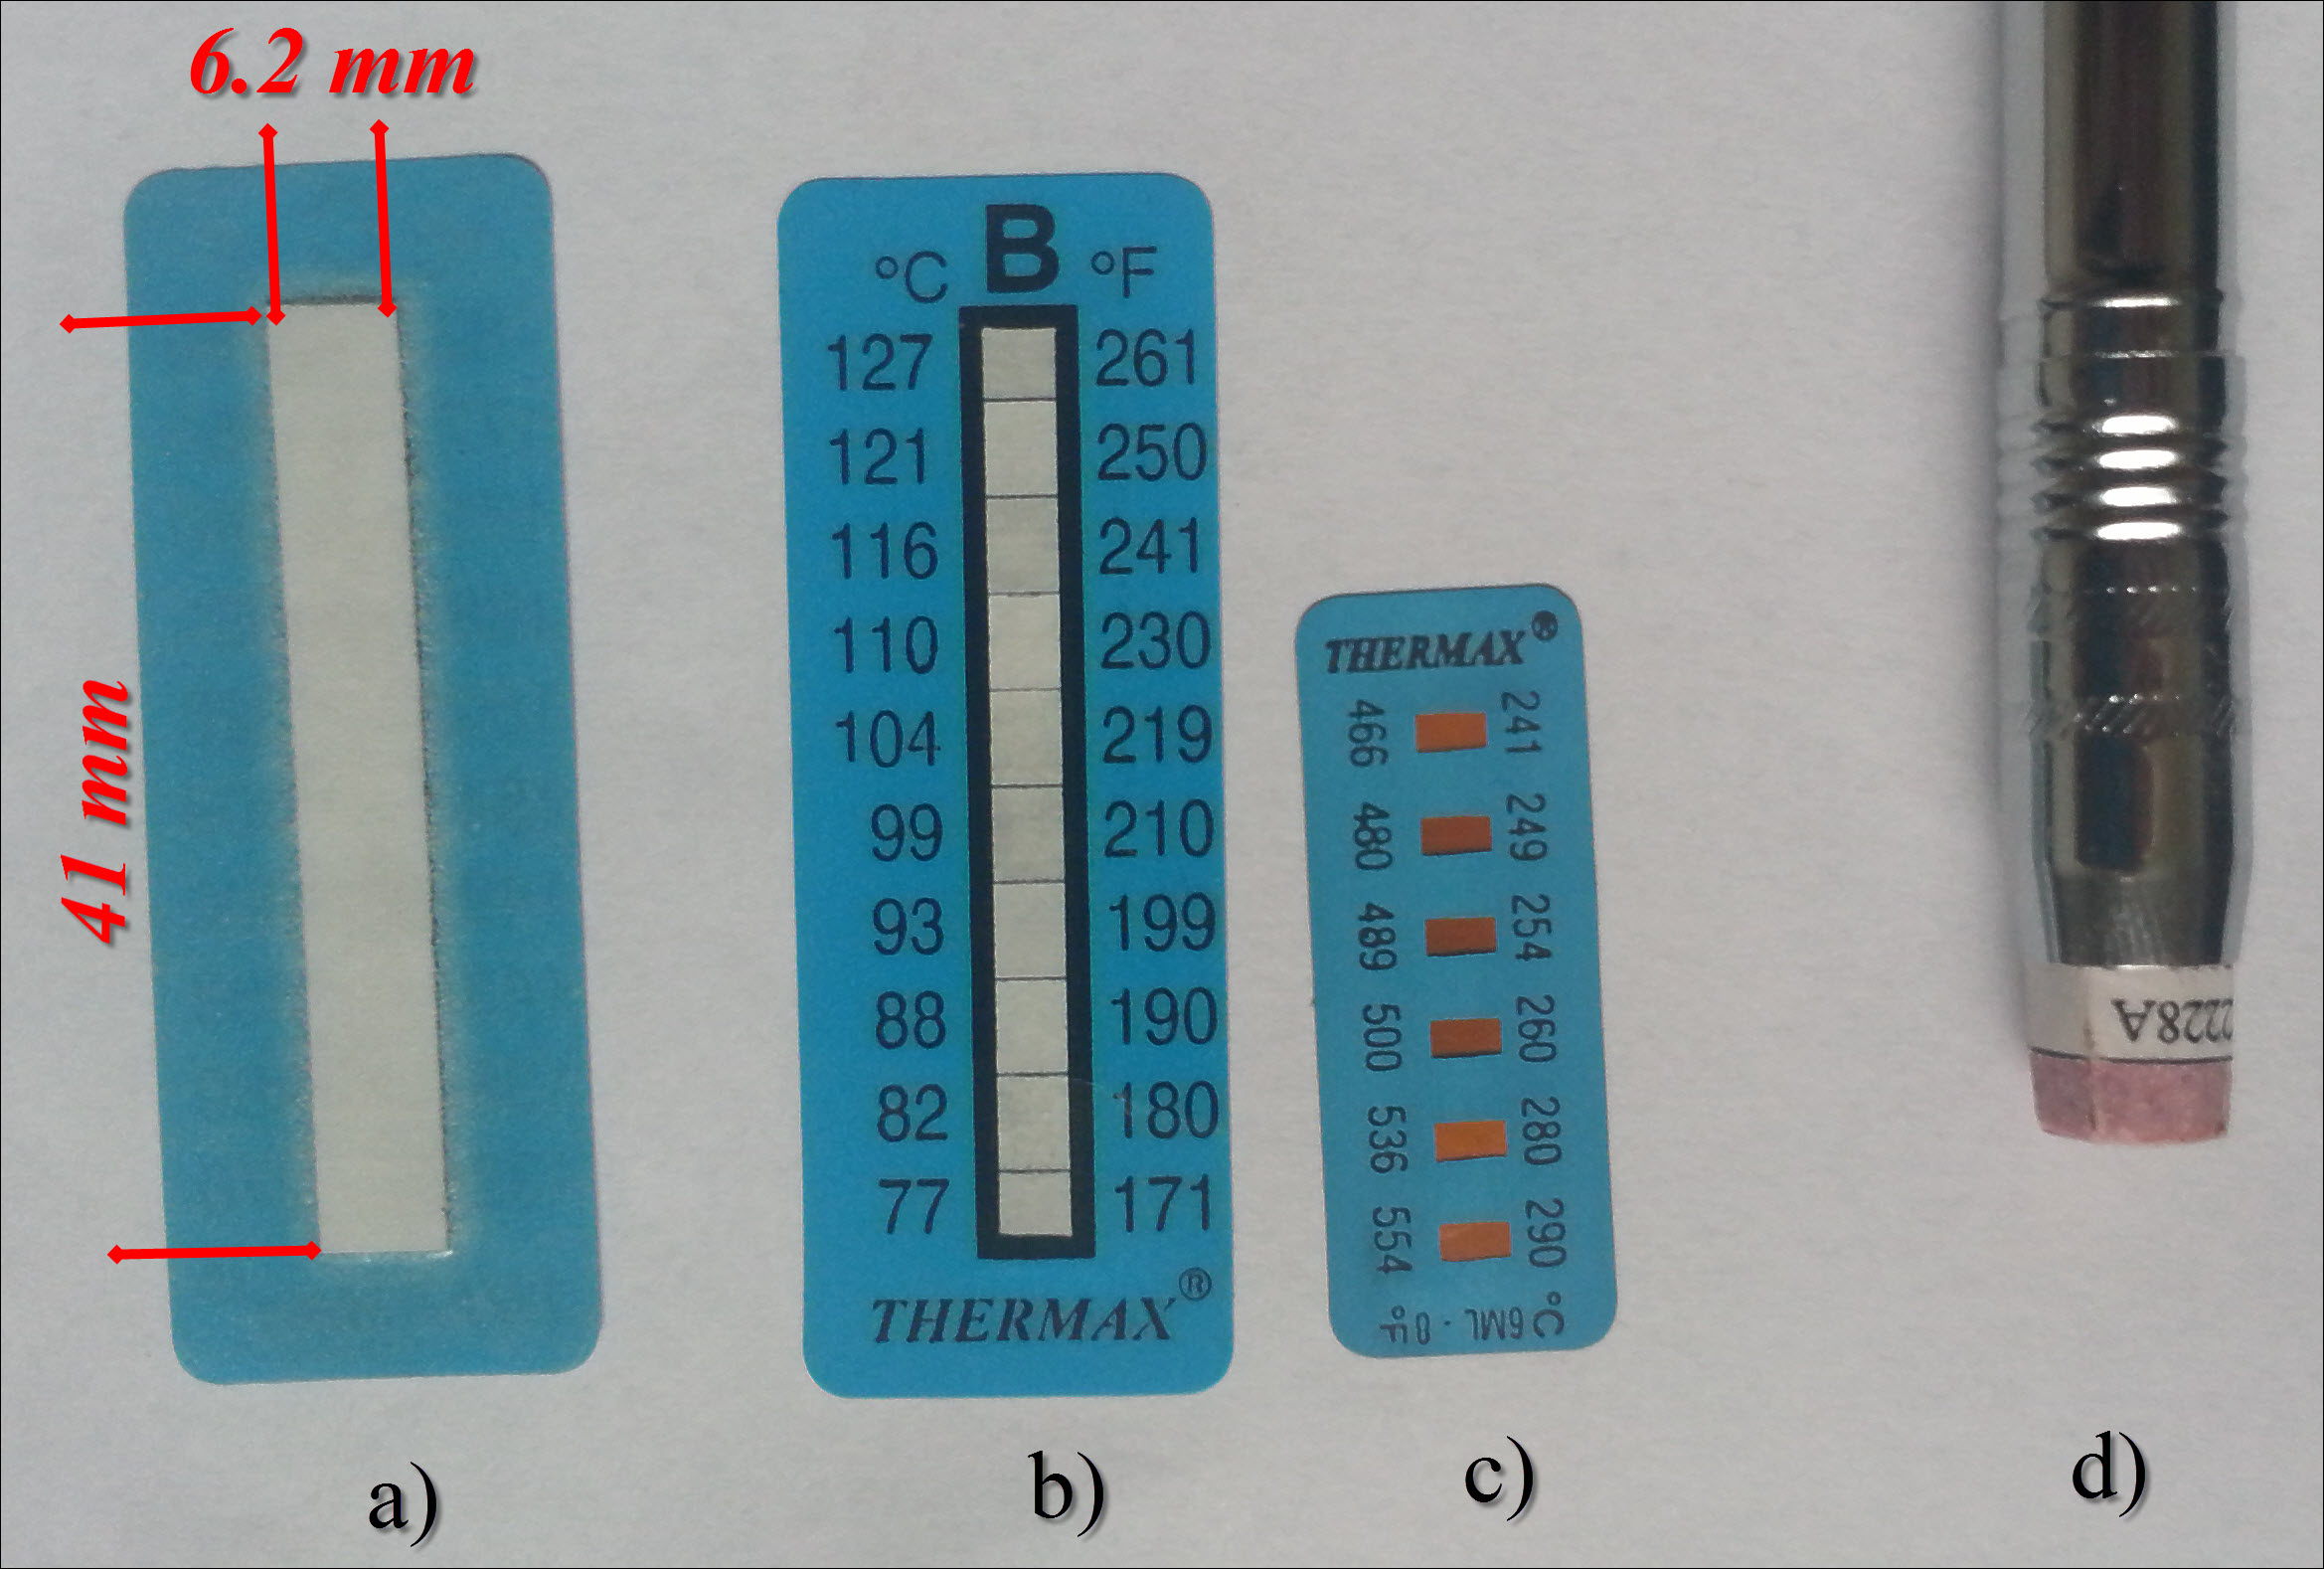
\includegraphics[width=.8\textwidth]{messstreifen}
\caption{a) - c) Verschiedene Messstreifen für verschiedene Temperaturbereiche , d) Schmelzkreide (\SI{205}{\degreeCelsius}) }
\label{fig:messstreifen}
\end{figure}
\begin{figure}[H]
\centering
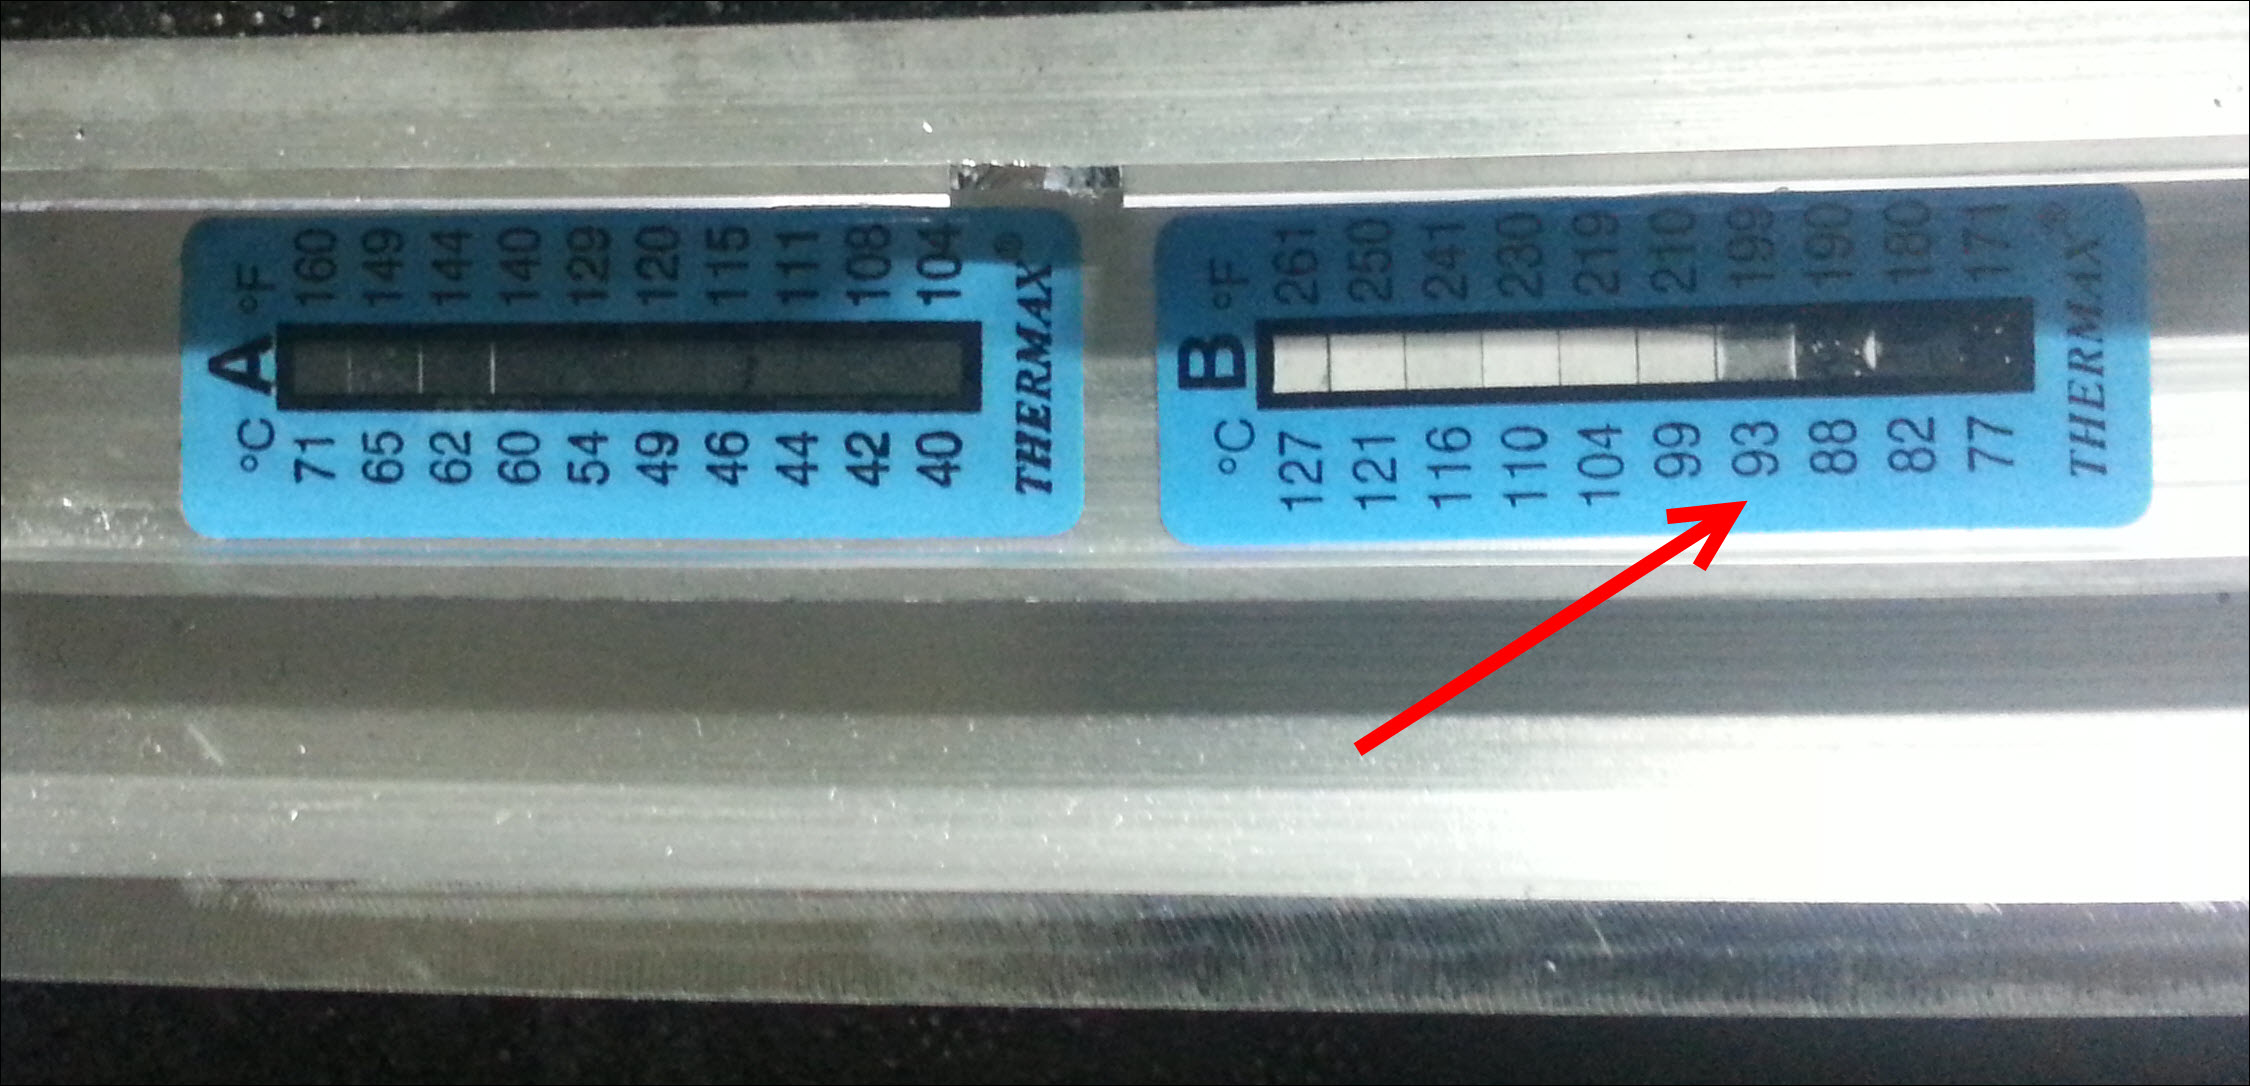
\includegraphics[width=.8\textwidth]{messaction}
\caption{Messstreifen mit Verfärbung Temperaturbereich}
\label{fig:messaction}
\end{figure}

Eine Übersicht der von den  Messstreifen abgedeckten Temperaturbereiche ist in folgender Tabelle zu sehen:

\begin{table}[H]
\caption{Messbereiche der Messstreifen}
\label{tab:messbereiche}
\centering
\begin{tabular}{ll}
\toprule
Messtreifen  & Temperaturbereich [\si{\degreeCelsius}]\\
\midrule
Typ A & 40-71\\
Typ B & 77-127\\
Typ C & 132-182\\
Typ D & 188-249\\
Typ 8 & 241-290\\
\bottomrule
\end{tabular}
\end{table}

Es sind sechs F17 Bauteile für die Versuchsserie mit den Messstreifen an jeweils drei Bereichen auf der Unterseite versehen worden.
\begin{figure}[H]
\centering
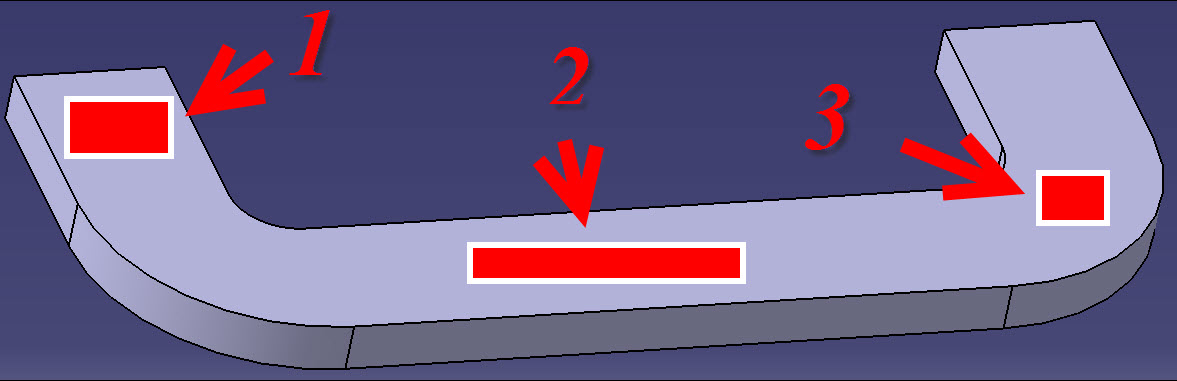
\includegraphics[width=.8\textwidth]{messbereicheVDKDunterseite}
\caption{Messzonen an Bauteilunterseite}
\label{messzonen}
\end{figure}

Nach dem Schleifvorgängen war keiner der Messstreifen verfärbt. Deshalb wird bei weiteren Betrachtungen nur noch der Polierprozess erwähnt. Nach dem Polieren der Proben wurden folgende Ergebnisse in einer Tabelle festgehalten und der Mittelwert (\SI{107.5}{\degreeCelsius}) ermittelt.



\begin{table}[H]
\caption{Messwerte nach dem Polieren}
\label{tab:messwerte}
\centering
\begin{tabular}{llll}
\toprule
              & \multicolumn{3}{c}{Temperatur [\si{\degreeCelsius}]}\\
              \cmidrule(ll){2-4}
 Charge/Nr. & Zone 1 & Zone 2 & Zone 3 \\
 \midrule
 F17 14 & 93 & 82 & 93 \\
 F17 15 & 99 & 93 & 82 \\
 F17 16 & 110 & 132 & 116 \\
 F17 17 & 99 & 127 & 104 \\
 F17 18 & 104 & 127 & 127 \\
 F17 19 & 104 & 127 & 116 \\
 \bottomrule             
\end{tabular}
\end{table}

Mit der auf der Oberfläche aufgetragenen Temperaturschmelzkreide ließ sich zwar schreiben, dennoch hatte sie sich nicht vollständig aufgelöst. Daraus folgt das zumindest kurz nach dem Entfernen des Bauteils aus der Polierzone auf der Oberfläche die \SI{205}{\degreeCelsius} nicht überschritten wurden. Hier ist jedoch zu beachten,  dass sich die Oberfläche (auch zusätzlich bedingt durch die kühlende Luft des rotierenden Polierringes) schnell abkühlt.

\begin{figure}[H]
\centering
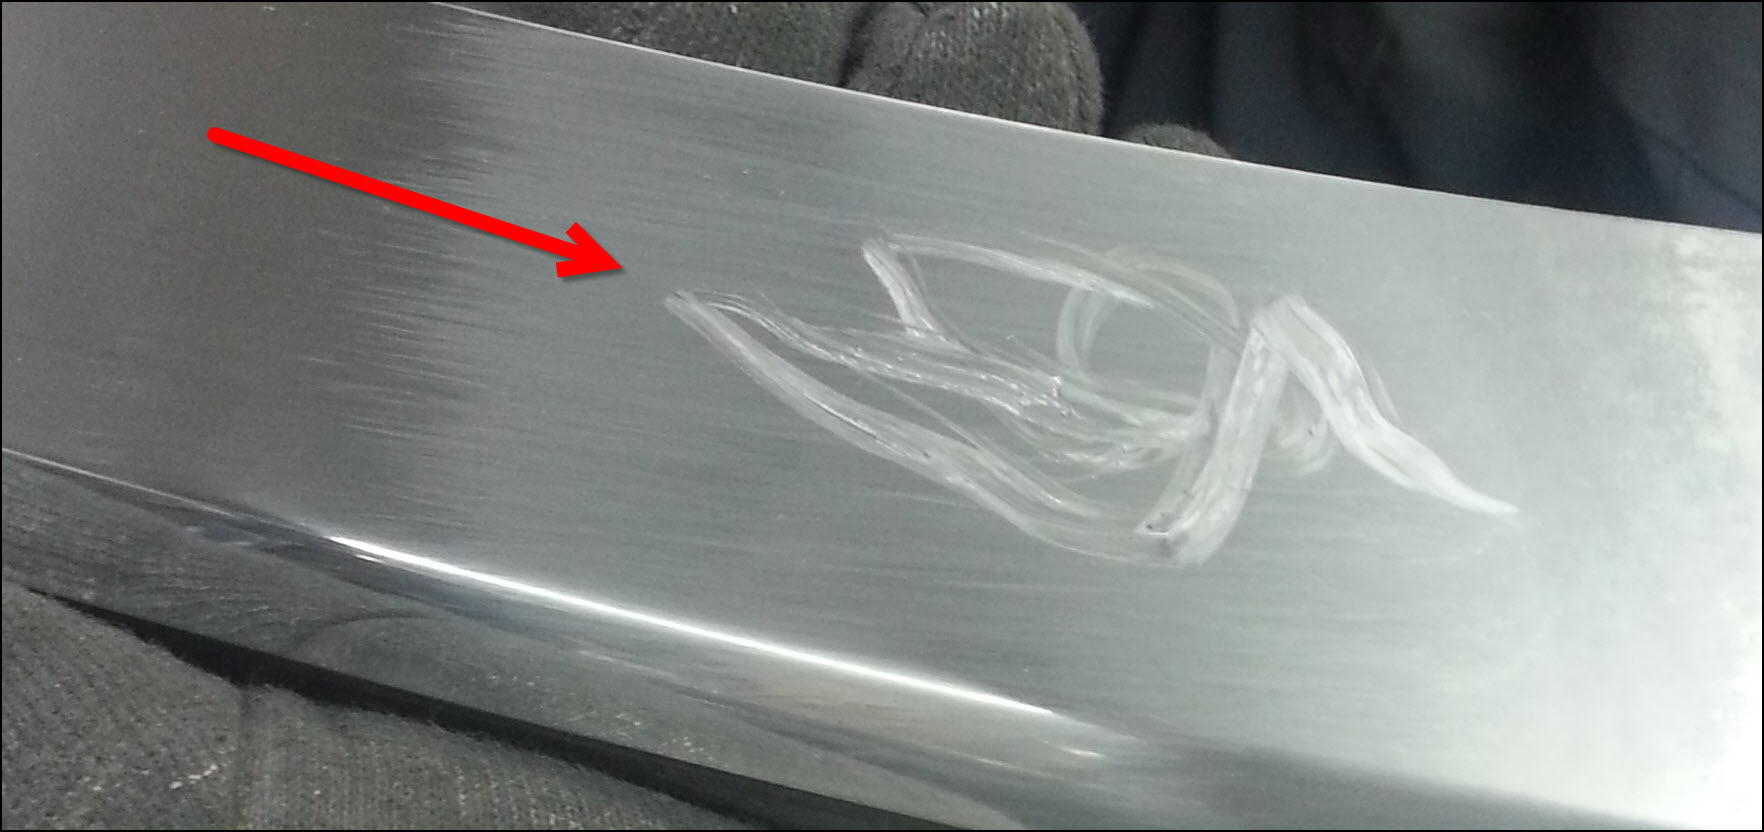
\includegraphics[width=.8\textwidth]{Kreide}
\caption{Direkt nach dem "`Wegschwenken"' der Oberfläche aus der Polierzone aufgetragene Temperaturschmelzkreide(\SI{205}{\degreeCelsius}). Nicht geschmolzen.}
\label{kreide}
\end{figure}









\subsubsection{Herleitung der Formel und Berechnung der Oberflächentemperatur}
Die metallurgischen Vorgänge in der Oberflächenzone bei dem Polierprozess sind sehr komplex. Auch die wirklichen Temperaturen in der Bearbeitungszone sind messtechnisch schwer zu erfassen. Eine Wärmekamera oder die Finite - Elemente - Methode wären aufschlussreicher, jedoch auch aufwendiger. Da das Polieren ein instationärer Prozess ist (Wärme wird zu unterschiedlichen Zeiten eingebracht, der ausgeübte Druck ist nicht gleichmäßig und variiert unter den Polierzonen aufgrund der unterschiedlichen Geometrien des Werkstücks, auch variierende Andruckkraft bei unterschiedlichen Personen um nur einige Parameter zu erwähnen) sind auch mathematische Herleitungen sehr theoretisch . Deshalb wird, um eine gute Annäherung der Oberflächentemperatur zu erhalten, vereinfachend von einem stationären Prozess bei der \emph{Wärmeleitung} durch eine ebene Wand ausgegangen.

\begin{figure}[H]
\centering
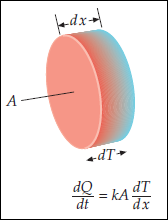
\includegraphics[width=.8\textwidth]{warmleittip}
\caption{Stationäre Wärmeleitung durch ebene Wand\protect\footnotemark}
\label{tipler}
\end{figure}  
\footnotetext{\cite[Vgl.][675]{phtip}}
Die unten vollzogene Näherungsrechnung ergab eine Oberflächentemperatur von \SI{175.69}{\degreeCelsius}. Ein Resultat was auch durchaus realistisch erscheint.
An dieser Stelle sei noch hinzugefügt, dass  bei modernen Roboterpolierzellen wesentlich höhere Temperaturen in der Materialoberfläche auftreten.



\newpage
\begin{description}
\item[ $\vartheta $] Temperatur  [\si{\degreeCelsius}]
\item[$ \dot{Q} $ ] Wärmestrom [\si{\watt}]
\item[$ \si{T}$] thermodynamische (auch absolute) Temperatur [\si{\kelvin
}]
\item[$\lambda $] Wärmeleitfähigkeit [\si{\watt\per\metre\per\kelvin}], ist in diesem speziellen Fall die Wärmeleitfähigkeit von Aluminium EN AW 6060 ($200-220 \, \si{\watt\per\meter\per\kelvin}$)\footnote{Vgl.\url{http://www.smh-metalle.de/internet/media/smh/pdf/datenblatt/datenblatt_en_aw_6060.pdf}[09.04.2014].}. In der Rechnung wird der Mittelwert (\SI{210}{\watt\per\meter\per\kelvin}) verwendet.
\item[$ P_{zu} $] Leistung [\si{\watt}], hier Leistung des Antriebs der Poliermaschine (Drehstrommotor)  \SI{9}{\watt}
\item[$P_{ab} $]  abgegebene Leistung [\si{\watt}] der Poliermaschine nach der Formel $ P_{ab} = P_{zu} \cdot \eta_{el.} \cdot \eta_{mech.}$.\footcite[Vgl.][R2]{g}
\item[$\eta_{el.} $] Wirkungsgrad des Drehstrommotors (Richtwert 0,85)\footcite[Vgl.][40]{tm}
\item[$\eta_{mech.} $]Wirkungsgrad des Breitkeilriemengetriebes der Poliermaschine (Richtwert 0,85)\footcite[Vgl.][40]{tm}
\item[$A_{mess} $] effektive Fläche des Messstreifens (siehe  a) in \fref{fig:messstreifen}) $ A_{mess} = \SI{6.2e-3}{\meter} \cdot \SI{4.1e-2}{\meter} = \SI{2.54e-4}{\meter\squared}$
\item[$x_a $]  Maß an Bauteil Außenwand (dort wo der Kontakt zum Polierring entsteht und die Wärme eintritt)[\si{\meter}]. 
\item[$x_i$] Maß Bauteil Innenwand ( Wärmeaustritt)[\si{\meter}]
\item[$\vartheta_a$] Temperatur Außenwand [\si{\degreeCelsius}] 
\item[$\vartheta_i$] Temperatur Innenwand [\si{\degreeCelsius}] hier Mittelwert der Messungen \SI{107.5}{\degreeCelsius} 
\item[$ \Delta x $] Blechdicke [\si{\meter}], hier \SI{2.8e-3}{\meter}

\end{description}

Herleitung der Formel\footcite[Vgl.][18-19]{wae} für die zu ermittelnde Oberflächentemperatur:

\begin{gather}
\dot{Q} = - \lambda \cdot A_{mess} \cdot \frac{d\vartheta}{dx}\\
\int\limits_{x_a}^{x_i} \dot{Q}\,dx = \int\limits_{\vartheta_a}^{\vartheta_i} - \lambda \cdot A_{mess}\,d\vartheta\\
\dot{Q} = \frac{\lambda}{x_i - x_a} \cdot A_{mess} \cdot (\vartheta_a - \vartheta_i) = \frac{\lambda}{\Delta x} \cdot A_{mess} \cdot (\vartheta_a - \vartheta_i)\\
P_{zu} \cdot \eta_{el.} \cdot \eta_{mech.} = \frac{\lambda}{\Delta x} \cdot A_{mess} \cdot (\vartheta_a - \vartheta_i)\\
\Rightarrow \quad  \vartheta_a = \frac{P \cdot \eta_{el.} \cdot \eta_{mech.} \cdot \Delta x}{\lambda \cdot A_{mess}} + \vartheta_i \\
\vartheta_a = \left(\frac{\SI{9e3}{\watt} \cdot 0.85 \cdot 0.85 \cdot \SI{2.8e-3}{\meter}}{\SI{210}{\watt\per\meter\per\kelvin} \cdot \SI{2.54e-4}{\meter\squared}}- \SI{273.15}{\kelvin}\right) \cdot \SI{1}{\degreeCelsius\per\kelvin} + \SI{107.5}{\degreeCelsius} \notag\\
\vartheta_a = \underline{\underline{\SI{175.69}{\degreeCelsius}}} \notag
\end{gather}

  







 
 





\printbibliography
\end{document} 
 
